\documentclass[aps,reprint,superscriptaddress,10pt]{revtex4-2}
\usepackage{kotex}
\usepackage[HWP]{dhucs-interword}
\usepackage[dvips]{color}
\usepackage{graphicx}
\usepackage{bm}
\usepackage{amsmath}
\usepackage{tikz}
\usepackage{mhchem}
\usepackage{booktabs}
\usepackage{multirow}
\usepackage{array}
\usepackage{tikz}
\usepackage{tabularx}

\begin{document}
\title{응집물질물리실험 결과보고서 \\
\small 실험주제 : Superconductivity, Hysteresis and Thermocouple}

\author{HuiJae-Lee}\email{hjlee6674@inha.edu}
\affiliation{Physics Department, Inha University}

\date{\today}

\begin{abstract}
  이번 실험을 통해 자성체의 Hysteresis 곡선이 코일에 인가된 전압 진폭, 주파수, 
  전압 파형에 따라 어떤 영향을 받는지 파악할 수 있었으며 열전대 현상으로 인한
  전압이 온도차에 따라 선형적으로 비례한다는 사실을 알 수 있었다.
  \end{abstract}

 \maketitle
 
 \section{Process}
 \subsubsection{Hysteresis of Transformer Core}
\begin{itemize}
  \item[1. ] 컴퓨터, 함수발생기, 코일 및 자성체, 연결선을 준비한다.
  \item[2. ] 컴퓨터를 키고 실험용 프로그램을 실행시킨다.
  \item[3. ] 함수발생기 및 각 키트를 연결선으로 연결하고 이를 다시 컴퓨터에 연결하여
  연결 상태를 확인한다.
  \item[4. ] 함수발생기의 입력 파형, 주파수, 전압 진폭을 바꿔가며 히스테리시스 곡선의
  형태를 측정하고 데이터를 저장한다.
  \item[5. ] 입력 파형(사인파, 삼각파, 사각파), 주파수(0.1 Hz, 0.2 Hz, 0.5 Hz), 
  전압 진폭(2V, 4V)을 바꿔가며 결과를 측정한다. 각 조건을 바꿀 때 마다
  자성체의 방향을 변경하여 자화된 상태의 영향을 덜 받도록 한다.
  \item[6. ] 얻은 데이터를 통해 결과를 분석한다.
\end{itemize}
\subsubsection{Calibrating of Thermocouple}
\begin{itemize}
  \item[1. ] 금속 도선, 온도계, 전압계, 핫플레이트, 얼음, 물, 비커를 준비한다.
  \item[2. ] 두 비커에 각각 물, 얼음을 채우고 온도계를 설치한다.
  \item[3. ] 물이 담긴 비커는 핫플레이트 위에 놓는다.
  \item[4. ] 금속 도선의 접합부를 두 비커 안에 두고 전압계에 연결한다.
  \item[5. ] 온도계의 눈금과 전압계의 전압을 기록한다.   
\end{itemize}

\newpage

\section{Result}

\subsubsection{Hysteresis of Transformer Core}

먼저 0.1Hz, 2V 조건에서 sine파형의 교류전원에 대한 Hysteresis 곡선은 다음과 같이
그려졌다.(FIG.~\ref{fig:sine,0.1,2})

\begin{figure}[htbp]
  \centering
  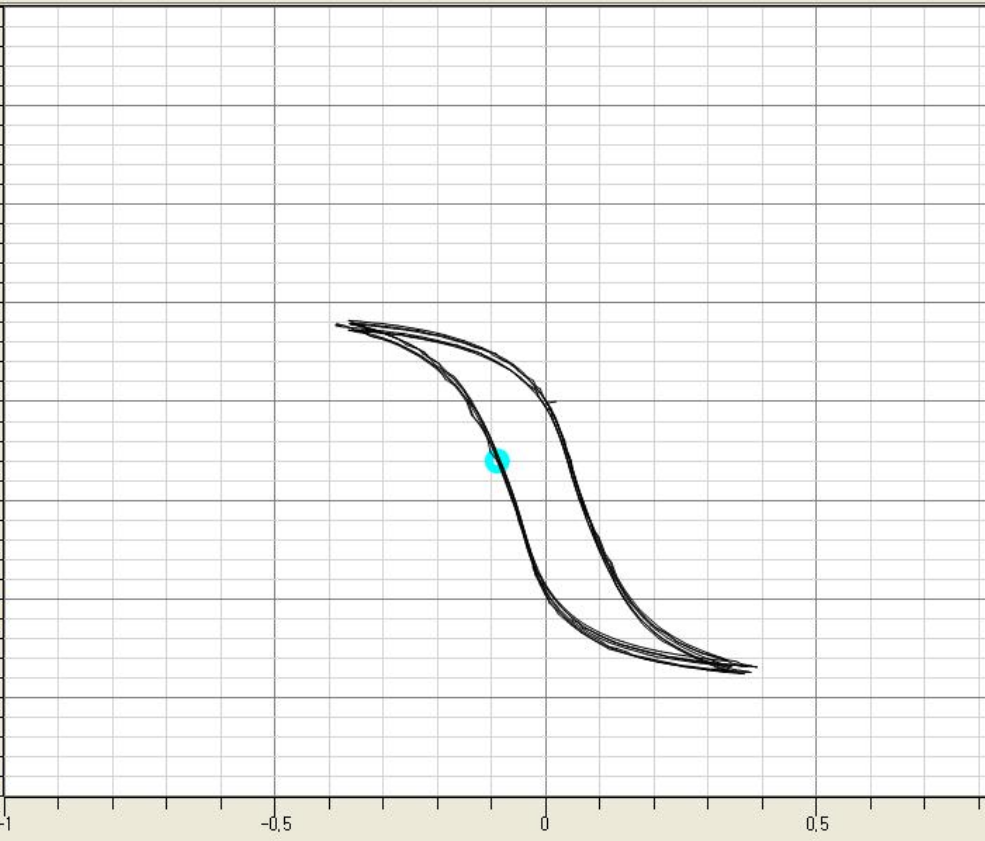
\includegraphics[scale = 0.15]{sine,0.1,2.png}
  \caption{0.1Hz, 2V 조건에서 sine파형의 교류전원에 대한 Hysteresis 곡선}
  \label{fig:sine,0.1,2}
\end{figure}

전압 진폭에 따른 Hysteresis 곡선의 변화를 측정하기 위해 전압 진폭만 4V로 높인 후
곡선을 측정하였다.(FIG.~\ref{fig:sine,0.1,4})
\begin{figure}[htbp]
  \centering
  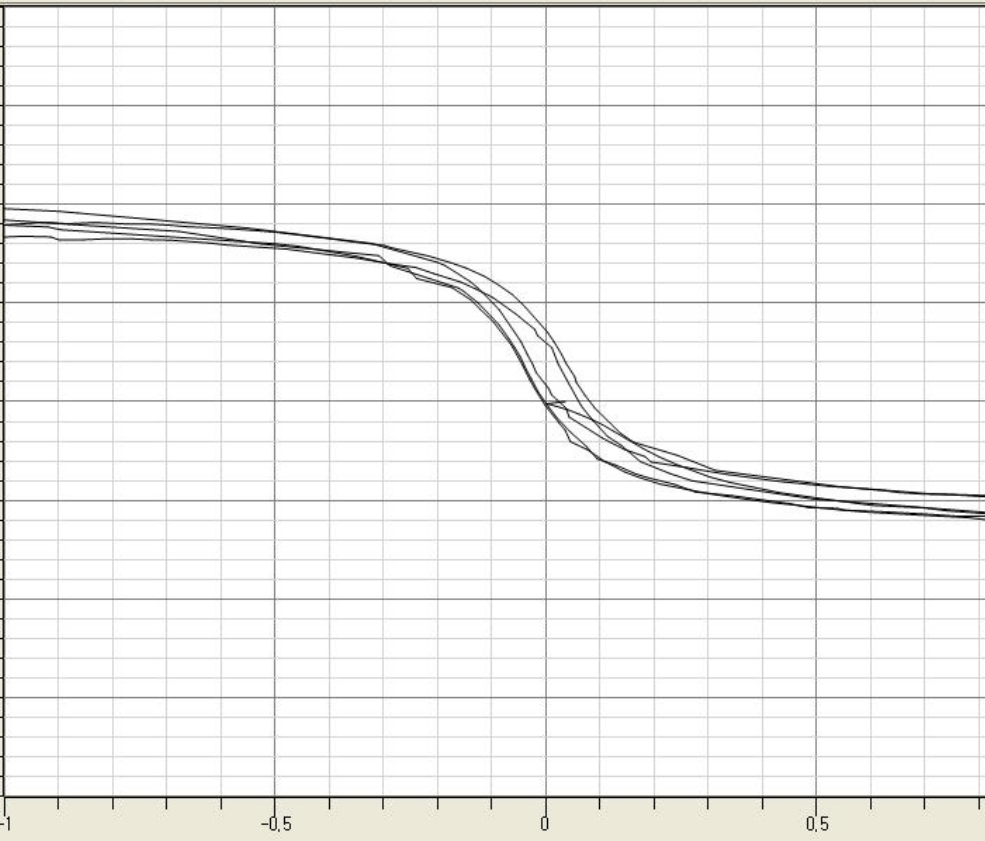
\includegraphics[scale = 0.15]{sine,0.1,4.png}
  \caption{0.1Hz, 4V 조건에서 sine파형의 교류전원에 대한 Hysteresis 곡선}
  \label{fig:sine,0.1,4}
\end{figure}
\newpage

교류전원의 주파수에 따른 Hysteresis 곡선의 변화를 측정하기 위해 2V, sine파형의
교류전원을 0.2Hz, 0.5Hz의 주파수로 코일에 인가하였다. 
(FIG.~\ref{fig:sine,0.2,2}, FIG.~\ref{fig:sine,0.5,2})
\begin{figure}[htbp]
  \centering
  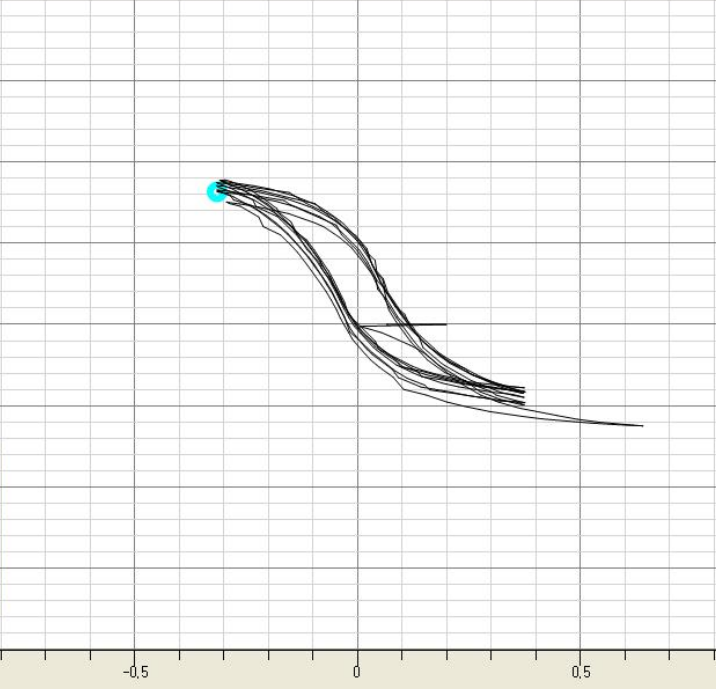
\includegraphics[scale = 0.175]{sine,0.2,2.png}
  \caption{0.2Hz, 2V 조건에서 sine파형의 교류전원에 대한 Hysteresis 곡선}
  \label{fig:sine,0.2,2}
\end{figure}

\begin{figure}[htbp]
  \centering
  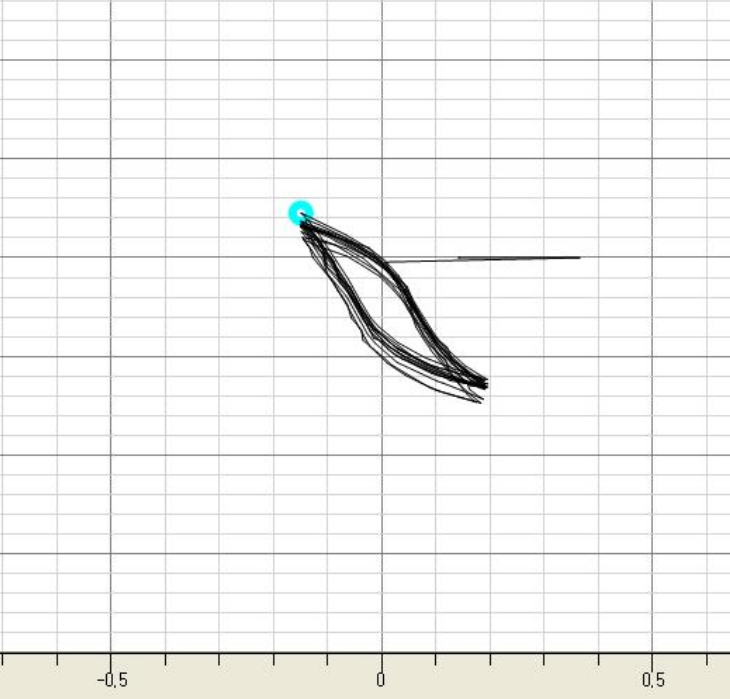
\includegraphics[scale = 0.175]{sine,0.5,2.png}
  \caption{0.5Hz, 2V 조건에서 sine파형의 교류전원에 대한 Hysteresis 곡선}
  \label{fig:sine,0.5,2}
\end{figure}

교류전원의 파형에 따른 Hysteresis 곡선의 변화를 측정하기 위해 0.1Hz, 2V의
교류전원을 sawtooth, sqaure 파형으로 코일에 인가하였다. 
(FIG.~\ref{fig:sawtooth,0.1,2}, FIG.~\ref{fig:square,0.1,2})

\begin{figure}[htbp]
  \centering
  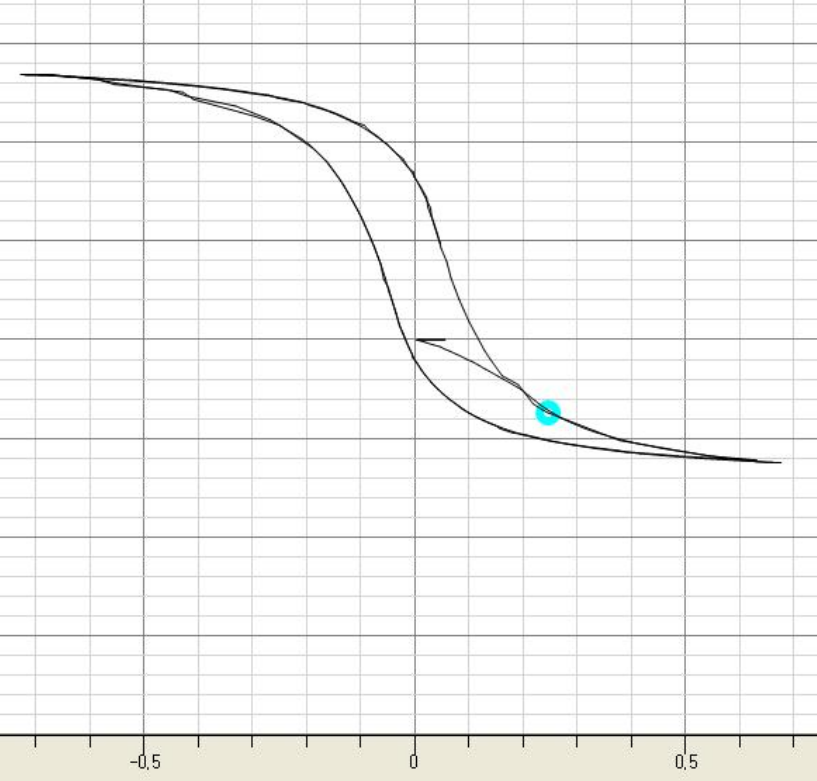
\includegraphics[scale = 0.2]{sawtooth,0.1,2.png}
  \caption{0.1Hz, 2V 조건에서 sawtooth파형의 교류전원에 대한 Hysteresis 곡선}
  \label{fig:sawtooth,0.1,2}
\end{figure}

\begin{figure}[htbp]
  \centering
  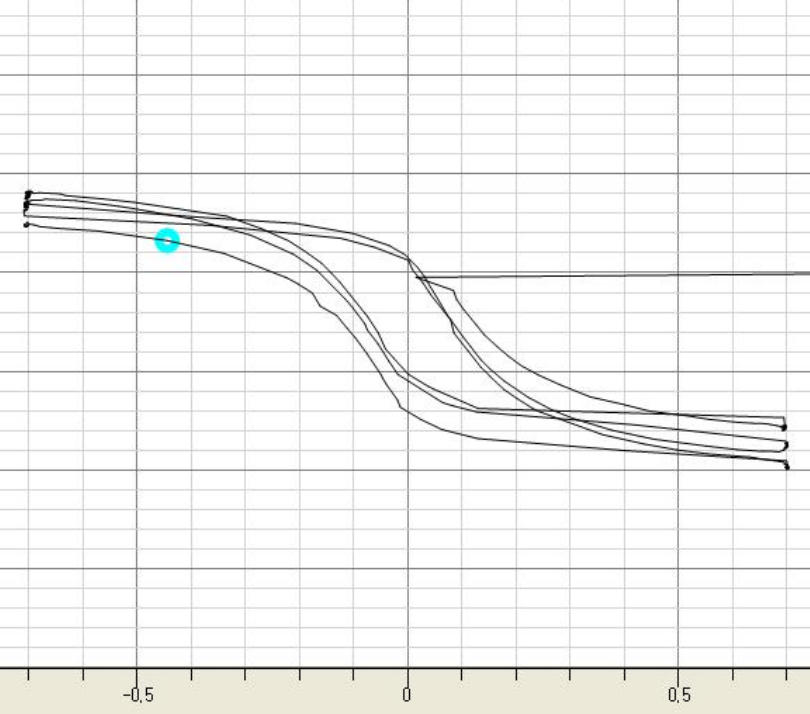
\includegraphics[scale = 0.2]{square,0.1,2.png}
  \caption{0.1Hz, 2V 조건에서 square파형의 교류전원에 대한 Hysteresis 곡선}
  \label{fig:square,0.1,2}
\end{figure}

\subsubsection{Calibrating of Thermocouple}
금속도선의 열전대 현상으로 인한 전위차 측정실험은 액체질소가 준비되어 있지 않았던
관계로 차가운 쪽에 상온의 물이 담긴 비커를 두어 실험을 진행하였다.
\begin{figure}[htbp]
  \centering
  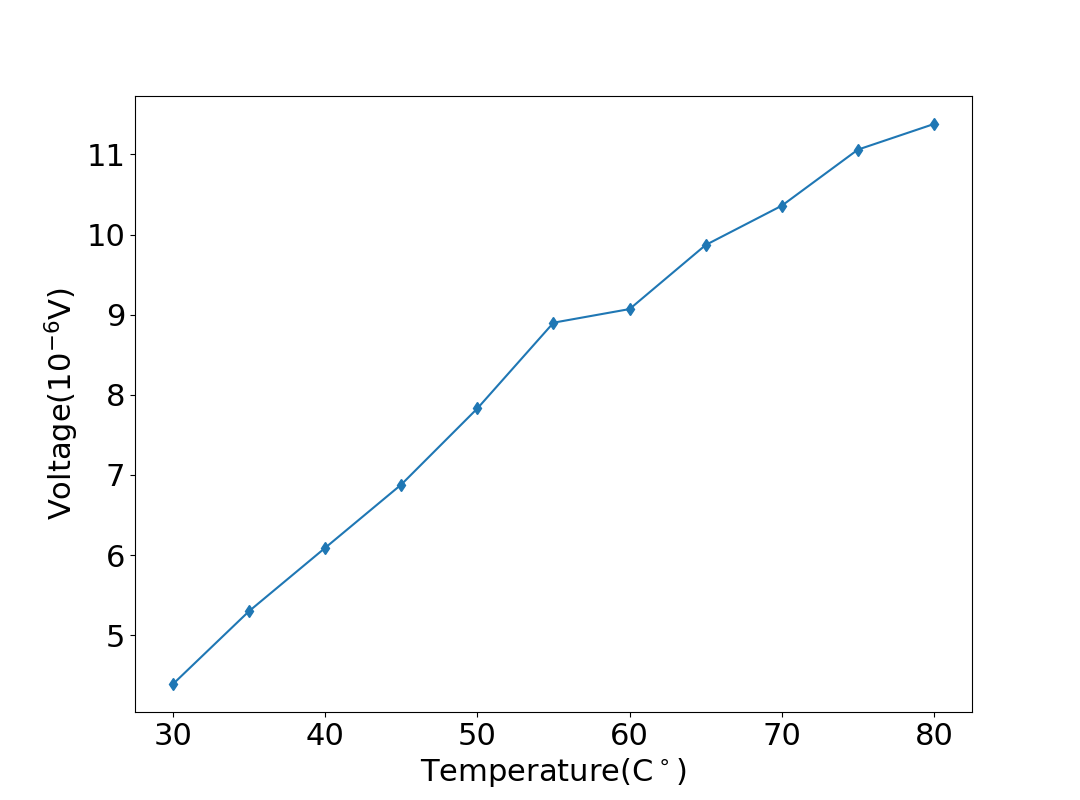
\includegraphics[scale = 0.3]{1124.png}
  \caption{금속도선의 온도에 따른 전압의 변화}
  \label{fig:1124}
\end{figure}

\section{Analysis}

\subsubsection{Hysteresis of Transformer Core}
\begin{itemize}
  \item[1. ] 전압 진폭에 따른 코일의 자화 상태를 Hysteresis 곡선의 비교를 통해 
  알아보기 위하여
  FIG.~\ref{fig:sine,0.1,2}와 
  FIG.~\ref{fig:sine,0.1,4}를
  비교해보면 전압 진폭을 증가시켰을 때 곡선이 좌우로 길게 늘어지는 것을 확인할 수 
  있다. 또한 세로축으로의 최댓값과 최솟값의 차이가 1.8 V로 유사하였다. 하지만
  전압 진폭이 4V일 때의 곡선이 2V일 때의 곡선보다 위로 평행이동한 모습을 보였다.
  이는 코일의 초기 조건에 의한 영향으로 보인다. 

  \item[2. ] 주파수에 따른 코일의 자화 상태를 Hysteresis 곡선의 비교를 통해 
  알아보기 위하여
  FIG.~\ref{fig:sine,0.1,2}와 
  FIG.~\ref{fig:sine,0.2,2}, FIG.~\ref{fig:sine,0.5,2}를
  비교해보면 주파수가 커질 수록 닫힌 곡선의 크기가 줄어든다는 사실을 확인할 수 있다.
  이는 주파수가 커지면 코일에 흐르는 전류의 방향이 빠르게 변해 코일의 자성체가
  최대로 자화되는 정도가 줄어들기 때문이다.
  

  \item[3. ] 주파수에 따른 코일의 자화 상태를 Hysteresis 곡선의 비교를 통해 
  알아보기 위하여
  FIG.~\ref{fig:sine,0.1,2}와 
  FIG.~\ref{fig:sawtooth,0.1,2}, FIG.~\ref{fig:square,0.1,2}를
  비교해보면 곡선이 좌우로 비교적 길어지며 곡선의 끝 부분에서 더 뾰족해진다는 사실을
  확인할 수 있다. 이는 파형이 sawtooth와 sqaure일 때 포화상태에 근접한 순간 sine보다 
  전압이 더 빠르게 변하기 때문이다. 또한 파형이 sqaure일 때 곡선의 끝 부분이 진하게
  나타나는 것을 볼 수 있는데 이는 자성체의 상태가 일정 시간 유지되었다는 것을 의미하며
  sqaure 파형이 전압을 일정한 최댓값에서 일정 시간 유지시킨다는 사실과 부합한다.
  
\end{itemize}



\subsubsection{Calibrating of Thermocouple}
FIG.~\ref{fig:1124}에서 확인할 수 있듯이 열전대에 의한 전위차는 온도 변화에 선형적으로
비례하며 온도 차가 커질 수록 전위차가 커진다는 사실을 알 수 있다. Seebeck coefficient를
구하기 위해 다음의 공식을 이용하자.
\begin{align}
  V = \alpha(T_1-T_2).
\end{align}
이 경우 낮은 온도 $T_2$는 16 $^\circ$C 이므로 각 온도차와 전압에 따른 $\alpha$의 평균값은
$2.28\times 10^{-7}$ V/K임을 구할 수 있다. 따라서 실험을 통해 구한
금속 도선의 Seebeck coefficient는 $2.28\times 10^{-7}$ V/K이다.
\section{Conclusion}
\begin{itemize}
  \item[1. ] Hysteresis 곡선이 각 요소로 부터 받는 영향을 고려해보았을 때,
  포화 상태는 전압 진폭과 주파수가 충분히 클 때 도달한다. 다만 전압 진폭이나
  주파수가 아무리 크더라도 자성체가 최대로 포화하는 지점이 존재한다.
  또한 square 파형의 경우로부터, Hysteresis 곡선의 끝 부분이 자성체의 포화 상태를
  의미함을 알 수 있다.
  \item[2. ] 열전대 현상으로 발생하는 금속 도선의 전위차는 금속 도선의 온도차에
  비례한다는 사실을 알 수 있다.
  
  
\end{itemize}


% \nocite{*} 
% \bibliography{ref}



%\begin{thebibliography}{9}
%\end{thebibliography}

\vfill
\end{document}